\documentclass[aps,prb,twocolumn,superscriptaddress,floatfix,longbibliography]{revtex4-2}

\usepackage[utf8]{inputenc}
\usepackage[spanish]{babel}
\usepackage{graphicx}
\usepackage{amsmath}
\usepackage{subcaption}
\usepackage{wrapfig} 
\usepackage[export]{adjustbox}

\usepackage{amsmath,amssymb} % math symbols
\usepackage{bm} % bold math font
\usepackage{graphicx} % for figures
\usepackage{comment} % allows block comments
\usepackage{textcomp} % This package is just to give the text quote '
%\usepackage{ulem} % allows strikeout text, e.g. \sout{text}

%Para disminuir el tamaño de los caption:
\usepackage[font={small}]{caption}

\usepackage[spanish]{babel}
%Para cambiar coma por punto en el modo math:
\decimalpoint

\usepackage{enumitem}
\setlist{noitemsep,leftmargin=*,topsep=0pt,parsep=0pt}

\usepackage{xcolor} % \textcolor{red}{text} will be red for notes
\definecolor{lightgray}{gray}{0.6}
\definecolor{medgray}{gray}{0.4}

\usepackage{hyperref}
\hypersetup{
colorlinks=true,
urlcolor= blue,
citecolor=blue,
linkcolor= blue,
bookmarks=true,
bookmarksopen=false,
}

% Code to add paragraph numbers and titles
\newif\ifptitle
\newif\ifpnumber
\newcounter{para}
\newcommand\ptitle[1]{\par\refstepcounter{para}
{\ifpnumber{\noindent\textcolor{lightgray}{\textbf{\thepara}}\indent}\fi}
{\ifptitle{\textbf{[{#1}]}}\fi}}
%\ptitletrue  % comment this line to hide paragraph titles
%\pnumbertrue  % comment this line to hide paragraph numbers

% minimum font size for figures
\newcommand{\minfont}{6}

% Uncomment this line if you prefer your vectors to appear as bold letters.
% By default they will appear with arrows over them.
% \renewcommand{\vec}[1]{\bm{#1}}

%Cambiar Cuadros por Tablas y lista de...
%\renewcommand{\listtablename}{Índice de tablas}
\renewcommand{\tablename}{Tabla}
\renewcommand{\date}{Fecha}

\usepackage[bottom]{footmisc} %para que las notas al pie aparezcan en la misma página



\begin{comment}

%Comandos de interés:

* Para ordenar el documento:
\section{Introducción}
\section{\label{sec:Formatting}Formatting} %label para luego hacer referencia a esa sección

\ptitle{Start writing while you experiment} %pone nombre y título al documento dependiendo de si en el header están los comandos \ptitletrue y \pnumbertrue

* Ecuaciones:
\begin{equation}
a^2+b^2=c^2 \,.
\label{eqn:Pythagoras}
\end{equation}

* Conjunto de ecuaciones:
\begin{eqnarray}
\label{eqn:diagonal}
\nonumber d & = & \sqrt{a^2 + b^2 + c^2} \\
& = & \sqrt{3^2+4^2+12^2} = 13
\end{eqnarray}

* Para hacer items / enumerar:
\begin{enumerate}
  \item
\end{enumerate}

\begin{itemize}
  \item
\end{itemize}

* Figuras:
\begin{figure}[h]
    \includegraphics[clip=true,width=\columnwidth]{pixel-compare}
    \caption{}
     \label{fig:pixels}
\end{figure}

* Conjunto de figuras:
(no recuerdo)


* Para hacer referencias a fórmulas, tablas, secciones, ... dentro del documento:
\ref{tab:spacing}

* Para citar
Elementos de .bib
\cite{WhitesidesAdvMat2004}
url
\url{http://www.mendeley.com/}\\

* Agradecimientos:
\begin{acknowledgments}
We acknowledge advice from Jessie Zhang and Harry Pirie to produce Fig.\ \ref{fig:pixels}.
\end{acknowledgments}

* Apéndice:
\appendix
\section{\label{app:Mendeley}Mendeley}

* Bibliografía:
\bibliography{Hoffman-example-paper}

\end{comment}

\begin{comment}

Plots y tablas en orden:

* Figura de los cilindros con los PT100, la resistencia de referencia, la fuente, el multímetro y la computadora simbolizando el software de adquisisción de datos.
* Figura de los cilindros con la lampartira, la fuente que le da tensión y el multímetro para medir esa tensión

* Tabla de dimensiones de los cilindros
(la copio de prácticos anteriores)

* Figura del equipo de algto vacío (bomba mecánica, difusora, tubos, bridas, cámara, 3 cilindros...)
* Figura sobre cómo determinar epsilon (pirómetro, termocupla apoyados sobre cilindro exterior sin vacío)

PLOT PPAL:
* T vs t mostrando un gráfico lindo donde se vea bien el transitorio y el estacionario

SUBPLOTS:
* T vs t mostrando qué pasa si hay un cortocircuito interno que hace que la lámpara no prenda (se ven T bajas)
* T vs t mostrando qué pasa si no ponemos el telgopor
* T vs t mostrando qué pasa si falla el vacío
* T vs t mostrando qué pasa en el cilindro externo cuando agregamos N2
* T vs t mostrando qué pasa cuando cambiamos la potencia de la lamparita sobre la marcha



Determinación del producto de ctes
* T vs P recta para calcular la pendiente relacionada con el producto de constantes

Determinación de epsilon
* Gráfico Epsilon vs P

Bibliografía:
* Agregar referencia a la tabla de calibración R vs T
* Agregar referencia a que sacamos los datos de las áreas de un práctico de años anteriores

\end{comment}



\begin{document}

% Allows to rewrite the same title in the supplement
\newcommand{\mytitle}{Resolución numérica de la ecuación Schrödinger para una barrera de potencial.}

\title{\mytitle}

\author{Pablo C$\mathrm{\hbar}$ehade \\
    \small \textit{pablo.chehade@ib.edu.ar} \\
    \small \textit{Física computacional, Instituto Balseiro, CNEA-UNCuyo, Bariloche, Argentina} \\
    \small \textit{2021/12/20}}


\begin{abstract}

Se resolvió numéricamente la ecuación de Schrödinger unidimensional empleando el método de Crank-Nicholson con la representación de Cayley para el operador de evolución temporal. Se empleó como condición inicial un paquete gaussiano y condiciones de borde nulas correspondientes a una caja con barreras de potencial infinito. En cuanto al potencial en la zona interior, se consideró en primer lugar potencial nulo y, en segundo lugar, una barrera de potencial finito. Se corroboró la conservación de la norma, consecuencia directa del uso de la representación de Cayley, y de la energía. También se analizó la evolución temporal de la función de onda, de la posición y momento lineal medios y de sus indeterminaciones y se caracterizó cualitativamente sus comportamientos en distintos instantes de tiempo en función del potencial y de la energía cinética inicial del paquete gaussiano.

\end{abstract}

\maketitle


\section{Introducción}

\begin{comment}
Análisis del error en E con epsilon:
k0 = 50*sqrt(2)*M_PI en presencia de barrera de potencial
tmax = 0.0002
Energía inicial E       Epsilon
49243.1 = (70.635 pi)^2     0.001
49396.9 = (70.746 pi)^2     0.0005
49446.1 = (70.781 pi)^2     0.0001
49447.7 = (70.782 pi)^2     0.00005
\end{comment}

\ptitle{Presentar Ec. De Sch}

Dada una partícula $\Psi(x,t)$ en un potencial $V(x)$, su dinámica cuántica está dada por la ecuación de Schrödinger \cite{Griffiths}. En una dimensión, esta es
\[i \hbar \frac{\partial \Psi}{\partial t} = - \frac{\hbar^2}{2m} \frac{\partial^2 \Psi}{\partial x^2} + V(x) \Psi = H \Psi \]
donde $i = \sqrt{-1}$ es la unidad imaginaria, $\hbar$ es la constante de Plank reducida, $m$ es la masa de la partícula y $H$ es el operador Hamiltoniano
\begin{equation}
H = - \frac{\hbar^2}{2m} \frac{\partial^2 }{\partial x^2} + V(x).
\label{eq:Hamilton}
\end{equation}
Por simplicidad de notación, de ahora en más se considerará $\hbar = 1$ y $m = 1/2$.
Otro modo de expresar dicha ecuación es
\begin{equation}
\Psi(x,t) = e^{-i(t-t_0)H} \Psi(x,t_0)
\label{eq:sol_formal}
\end{equation}
donde el operador unitario $e^{-i(t-t_0)H}$ es el operador de evolución temporal y $t = t_0$ corresponde a la condición inicial $\Psi(x,t_0)$ conocida. Esta ecuación diferencial en derivadas parciales se puede resolver analíticamente sólo para determinados potenciales, como es el caso del potencial armónico, por ejemplo. Para otros existen a modo general dos alternativas: introducir aproximaciones y obtener una solución analítica aproximada o integrar numéricamente. En el presente trabajo se optó por este último camino.

El análisis de la evolución del sistema se puede realizar a partir del comportamiento de $\mid \Psi(x,t) \mid^2$ y de distintos observables. En cuanto a estos últimos, a modo general, dado un observable $Q(X, p, t)$ con $p = -i\hbar\frac{\partial}{\partial x}$, su esperanza $\langle Q \rangle$ se calcula como \cite{Griffiths}
\[\langle Q \rangle \equiv \langle \Psi \mid Q \mid \Psi \rangle \equiv \int{\Psi(x,t)^* Q(x, p, t) \psi(x,t)} \, dx \]
y su indeterminación o dispersión,
\begin{equation}
\sigma_Q = \sqrt{\langle Q^2 \rangle - \langle Q \rangle^2}
\label{eq:dispersion}
\end{equation}

\section{Métodos}

\ptitle{Representación de Carley y deducción de la expresión implícita}

En el esquema numérico, tiempo y espacio se encuentran discretizados a través de una red de tamaño $T \times L$ con unidad mínima $\delta$ y $\epsilon$, respectivamente.
\begin{comment}
De este modo, si $t$ varía entre $0$ y $t_{\mathrm{max}}$, el tiempo en unidades de $\epsilon$ varía entre $0$ y $N = t_{\mathrm{max}}/N$. Análogamente, si $x$ varía entre $0$ y $L$, en unidades de $\delta$ varía entre $0$ y 
\end{comment}
En base a esto, la ecuación \ref{eq:sol_formal} es equivalente a
\begin{equation}
\Psi_j^{n+1} = e^{-i\delta H} \Psi_j^n
\label{eq:Sch_sol_gral}
\end{equation}
donde $\Psi_j^n = \Psi(x = \epsilon j, t = \delta n)$, $j = 0, 1, \ldots, J = L/\epsilon$, $n = 0, 1, \ldots, N = T/\delta$ y $e^{-i\delta H}$ es el operador de evolución temporal discretizado. Para resolver esta ecuación es necesaria una discretización del mismo que sea estable numéricamente y unitaria, de modo de asegurar la normalización de la función de onda durante la evolución temporal. Con este fin se empleó la representación de Cayley
%\begin{equation}
%\label{eq:Cayley}
%\end{equation}
\[e^{-i\delta H} \Psi_j^n \approx \frac{1 - \frac{1}{2} i \delta H}{1 + \frac{1}{2} i \delta H} \]
que es $o(\delta^2)$. En cuanto al operador $H$ expresado en \ref{eq:Hamilton} se emplearon diferencias finitas centradas en el espacio para calcular la derivada de segundo orden $\frac{\partial^2}{\partial x^2}$, método de orden $o(\epsilon^2)$. Por lo tanto,
\begin{equation}
H \Psi_j^n \approx -\frac{1}{\epsilon^2}(\Psi_{j+1} - 2 \Psi_j + \Psi_{j-1}) + V_j \Psi_j
\label{eq_Hamilton_numerico}
\end{equation}
donde $V_j = V(x = \epsilon j)$. Aplicando estas aproximaciones a la ecuación \ref{eq:Sch_sol_gral} se obtiene
\begin{multline}
\Psi_{j+1}^{n+1} + (i \lambda - \epsilon^2 V_j - 2 ) \Psi_j^{n+1} + \Psi_{j-1}^{n+1} = \\ -\Psi_{j+1}^n + (i \lambda + \epsilon^2 V_j + 2) \Psi_j^n - \Psi_{j-1}^n,
\label{eq:Crank-Nicolson}
\end{multline}
donde $\lambda = 2 \epsilon^2/\delta$. La expresión obtenida corresponde al esquema de Crank-Nicolson para la ecuación de Schrödinger.

\ptitle{Método de Crack-Nicholson. Presentar bases de la aproximación (condiciones de borde) y resultado final. Mencionar que está detallado el procedimiento en el Goldberg}
El método de Crack-Nicholson es un método implícito, es decir, a partir de \ref{eq:Crank-Nicolson} no es posible despejar $\Psi^{n+1}$ en términos de $\Psi^n$ . Se requieren técnicas algebraicas para resolverlo. Estas se desarrollan en gran detalle en \cite{Goldberg} para condiciones de borde nulas $\Psi^n_0 = \Psi^n_J = 0$ $\forall n$, las cuales corresponden a barreras de potencial infinito en $x = 0$ y $x = L$ y son útiles para analizar cualquier potencial $V(x)$ siempre que la función no sea apreciable en las cercanías de los bordes. En otras palabras, las condiciones de borde elegidas implican potenciales que cumplen: $V(x) = \infty$ para $x<0$ y $x>L$. Pero si se quieren estudiar potenciales generales $V(x)$, basta con asegurar que durante la evolución temporal la función de onda $\Psi(x,t)$ no se aproxime a los bordes y, de este modo, no se vea afectada por el potencial infinito. Por completitud, se presentan a continuación las ecuaciones generales que permiten calcular $\Psi^{n+1}_j$ bajo las condiciones antes mencionadas:

\[\Psi_j^{n+1} = \frac{\Psi_{j+1}^{n+1} - f_j^n}{e_j}\]
donde
\begin{equation}
\begin{split}
\nonumber&f_j^n = \Omega_j^n + \frac{f_{j-1}^n}{e_{j-1}}, \\
\nonumber&\Omega_j^n = - \Psi_{j+1}^n + (i \lambda + \epsilon^2 V_j + 2) \Psi_j^n - \Psi_{j-1}^n, \\
\nonumber&e_j = 2 + \epsilon^2 V_j - i \lambda - \frac{1}{e_{j-1}}
\end{split}
\end{equation}
con
\begin{equation}
\begin{split}
\nonumber&f_1^n = \Omega_1^n, \\
\nonumber&e_1 = 2 + \epsilon^2 V_1 - i \lambda \\
\end{split}
\end{equation}

\ptitle{Parámetros del problema: condición inicial (fórmula y figura), condiciones de borde, parámetros del método numérico.}

En cuanto al potencial, se consideró una barrera de potencial
\[
V(x) = \left\{\begin{matrix}
U_0 & \mathrm{si \,\, \mid x - L/2 \mid < a} \\
0 &  \mathrm{si \,\, \mid x - L/2 \mid > a} 
\end{matrix}\right.
\]
donde $2 a$ es el ancho de la barrera y $U_0$ la altura de la misma. Como condición inicial se empleó un paquete de ondas gaussiano con momento $k_0 > 0$, centrado en $x_0 \in [0,L]$
\[ \Psi(x,0) = Ce^{i k_0 x} e^{-\frac{(x-x_0)^2}{4\sigma_0^2}}, \]
donde $C$ es la constante de normalización que se calcula numéricamente y $\sigma_0$ es una constante que da idea del ancho de la distribución a tiempo inicial. La distribución $\mid\Psi(x,0)\mid^2$ se grafica en la figura \ref{fig:condicion_inicial}, donde se agregó además un punto cuya coordenada horizontal representa $\langle x \rangle(0)$, y una flehca cuyo módulo representa $\langle p \rangle(0)$ normalizado a tiempo inicial. La energía inicial se calcula a partir de la expresión
\begin{equation}
E = (\hbar k_0)^2,
\label{eq:energia}
\end{equation}
válida siempre que la función de onda no sea apreciable en las zonas donde el potencial $V(x)$ es no nulo.

\begin{figure}[h]
    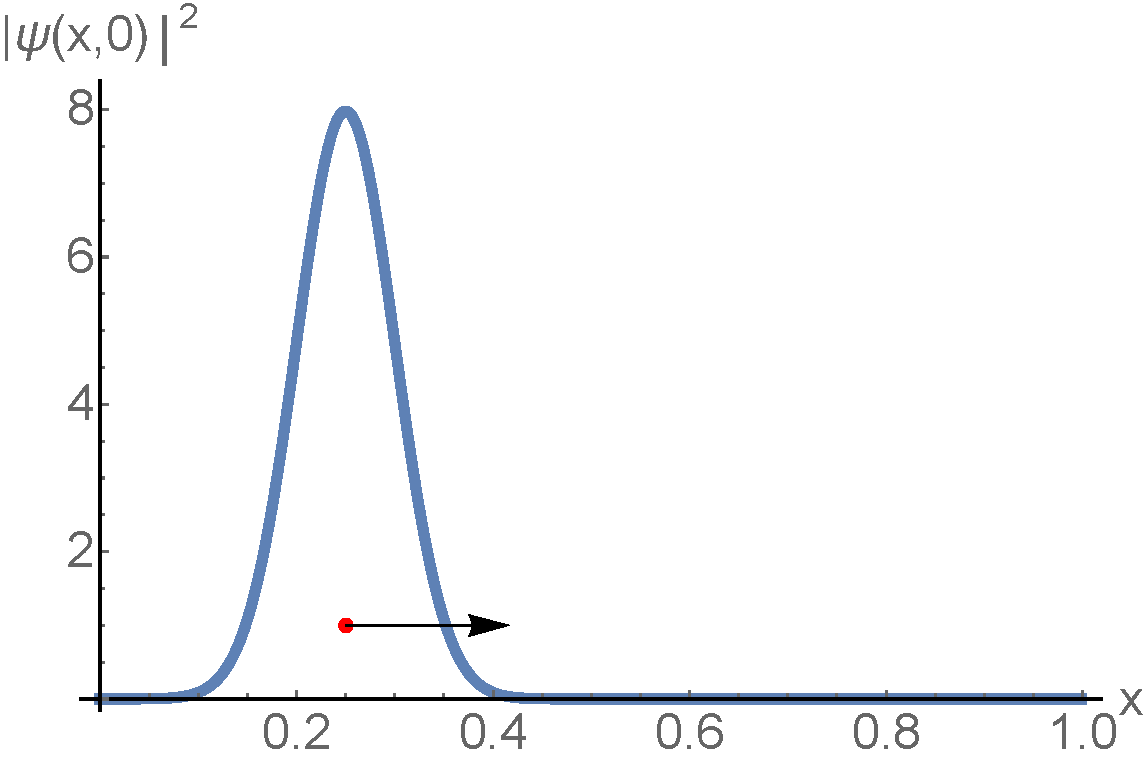
\includegraphics[clip=true,width=0.9\columnwidth]{condicion_inicial.pdf}
    \caption{Condición inicial $\mid \Psi(x,0) \mid^2$: paquete de onda gaussiano centrado en $x_0 = 0.25$ y ancho $\sigma_0 = 0.05$.}
     \label{fig:condicion_inicial}
\end{figure}

\ptitle{Qué casos se estudiaron}

Se resolvió numéricamente la ecuación de Schrödinger sobre una grilla discreta de tamaño $L = 1$ y $T \lesssim L/(2 \hbar k_0)$ con discretización temporal $\delta = 2 \epsilon^2 / \hbar = 2*10^{-6}$ y discretización espacial  $\epsilon = 0.001 \hbar = 0.001$. Se analizaron cuatro situaciones. En primer lugar, una partícula en ausencia de barrera de potencial ($U_0 = 0$) con condición inicial dada por $x_0 = 0.25$, $\sigma_0 = 0.05$ y $k_0^0 = 25 \pi$ que en base a la expresión \ref{eq:energia} tiene energía $E_1 = (25 \pi)^2$. En segundo lugar, una partícula sujeta a una barrera de potencial con parámetros $a = 0.032$ y $U_0 = (50 \pi)^2$ con condición inicial dada por los mismos valores de $x_0$ y $\sigma_0$ pero con distintos valores de momento $k_0$. Se consideró $k_0^1 = 25 \pi$, $k_0^2 = 35 \sqrt{2} \pi$ y $k_0^3 = 50 \sqrt{2} \pi$ correspondientes a energías iniciales $E_1 = E_0 = (25 \pi)^2 < U_0$, $E_2 \approx (49.5 \pi)^2 \lesssim U_0$ y $E_3 \approx (70.7 \pi)^2 > U_0$.

\ptitle{Cálculo de esperanzas: fórmula gral y aproximaciones usadas para calcular p y $p^2$.}

Durante la evolución temporal se corroboró la conservación de la norma $N = \int_0^L{\mid \Psi(x,t) \mid^2} \, dx$ y del valor medio de la energía $E(t) = \langle H \rangle = \langle K \rangle + \langle V \rangle$ con $K = p^2/2m$ energía cinética. Además, se analizó gráficamente $\mid \Psi(x,t) \mid^2$ calculado a partir de la representación discreta $\mid \Psi \mid_{j}^n = (\Psi_j^n)^* \Psi_j^n$ y se estudió la dependencia temporal de ciertos observables y sus indeterminaciones calculadas a partir de \ref{eq:dispersion}. Tal es el caso de la posición media $\langle x \rangle$, el momento medio $\langle p \rangle$ y sus dispersiones $\sigma_x$ y $\sigma_p$, respectivamente. Para este último se calculó numéricamente la derivada de primer orden $\frac{\partial}{\partial x}$ empleando diferencias finitas centrada
\[\frac{\partial \Psi}{\partial x} \approx \frac{ \Psi_{j+1} - \Psi_{j-1}}{2 \epsilon}\]
que es orden $o(\epsilon^2)$ y la derivada de segundo orden $\frac{\partial^2}{\partial x^2}$, empleando diferencias finitas centrada de igual manera que en la expresión \ref{eq_Hamilton_numerico}. Todas las integrales fueron realizadas empleando la regla del trapecio compuesta que es $o(\epsilon^2)$.


\begin{comment}
\ptitle{Principio de incerteza}


A modo de verificación, . Por último, se verificó el cumplimiento del principio de incertidumbre de Heisenberg \cite{Griffiths}
\begin{equation}
\delta x \delta p \geqslant \frac{\hbar}{2}
\label{eq:ppio_incer}
\end{equation}
determinando una cota inferior para todas las condiciones iniciales y ambos potenciales.
\end{comment}

\section{Resultados y discusión}

\ptitle{Conservación de la norma y de la energía}

En cuanto a la dependencia temporal de la norma, se obtuvo en todos los casos $N = 1$ $\forall t$. Esto se muestra gráficamente para el caso $U_0 = 0$ en la figura \ref{fig:norma}. La conservación de la norma es consecuencia directa de la unitariedad de la representación de Cayley, como se mencionó en la sección anterior.

\begin{figure}[h]
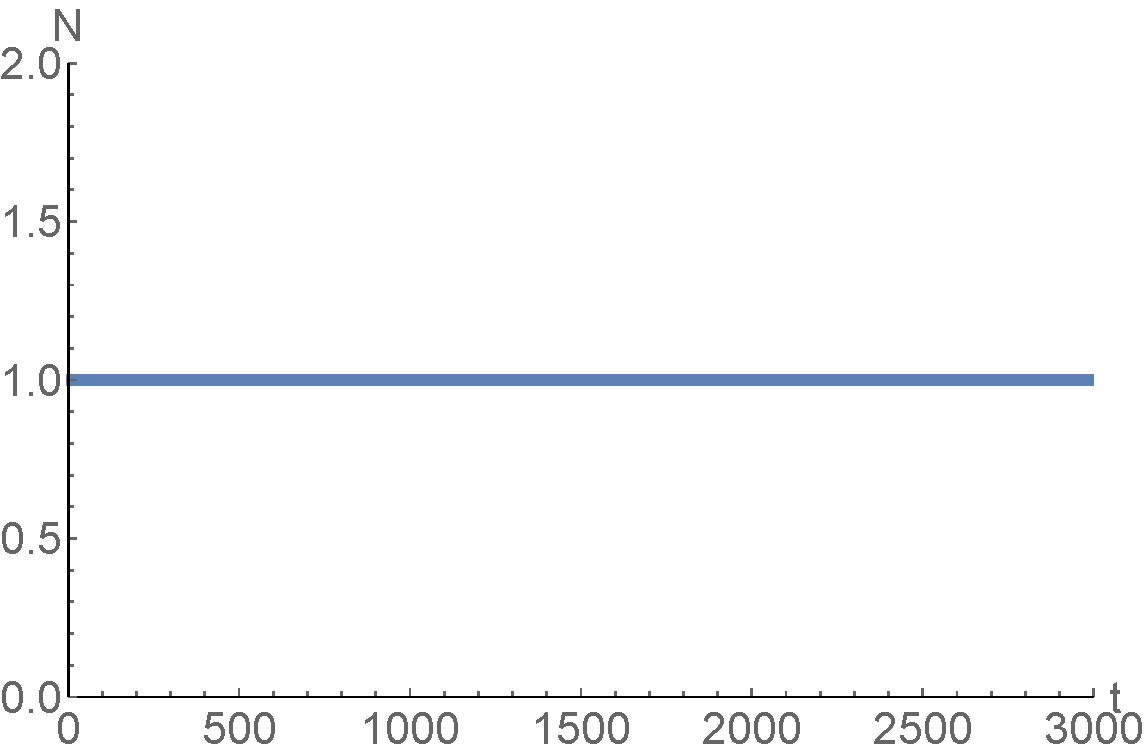
\includegraphics[clip=true,width=0.85\columnwidth]{norma.pdf}
\caption{Conservación de la norma $N$ en función del tiempo $t$ expresado en unidades de $\delta$ para el caso particular $U_0 = 0$.}
 \label{fig:norma}
\end{figure}

En cuanto a la dependencia temporal de la energía, se obtuvo en todos los casos la conservación de la misma, como se observa en la figura \ref{fig:energia}. Se obtuvo para la partícula en ausencia de barrera $E_0 = (25.2 \pi)^2$ y para las partículas en presencia de barrera, $E_1 = (25.2 \pi)^2$, $E_2 = (49.6 \pi)^2$ y $E_3 = (70.6 \pi)^2$. A partir de estos resultados se pueden obtener dos conclusiones. En primer lugar, se cumple lo buscado incialmente: $E_1 < U_0$, $E_2 \lesssim U_0$ y $E_3 > U_0$. En segundo lugar, no se cumple con exactitud la relación \ref{eq:energia}. Esto se puede deber a la discretización del sistema, esperando que a medida que $\delta$ y, principalmente, $\epsilon$ disminuyan, los valores medios de energía calculados se aproximen a los valores teóricos. Se necesitan realizar mayores estudios al respecto.

\begin{figure}[h]
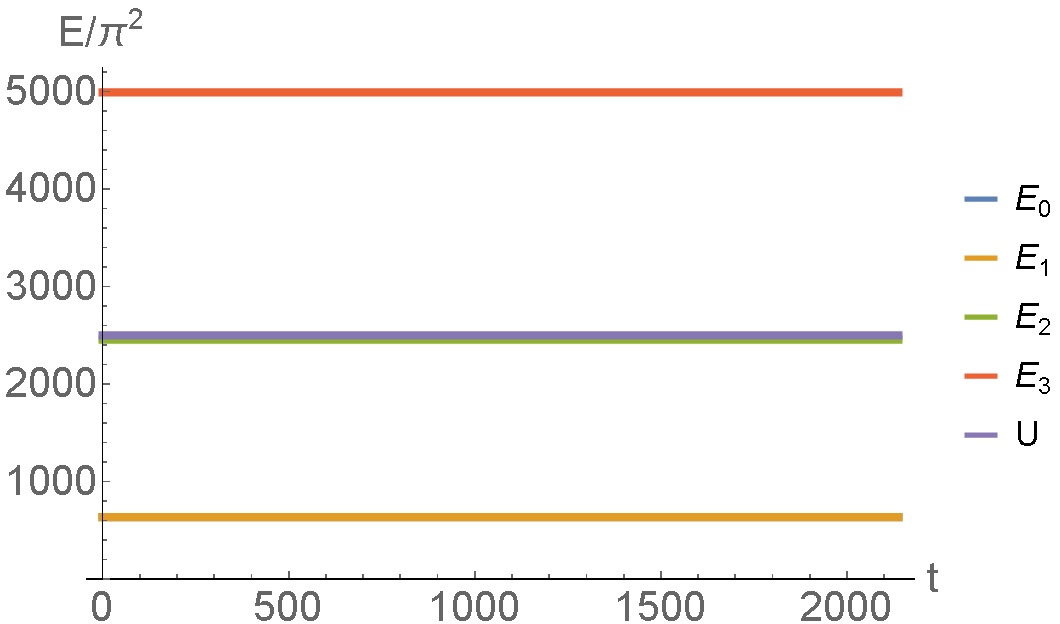
\includegraphics[clip=true,width=\columnwidth]{energia.png}
\caption{Conservación de la energía $E$ en función del tiempo $t$ expresado en unidades de $\delta$ para cuatro situaciones. $E_0$ corresponde a una partícula en ausencia de barrera de potencial. $E_1$, $E_2$ y $E_3$ corresponden a una partícula en presencia de barrera de potencial $U_0$ con distintos momentos $k_0$ inicial. Las curvas de $E_0$ y $E_1$ se encuentran encimadas.}
 \label{fig:energia}     
\end{figure}


\begin{comment}
Valores sin aproximar:
\[1. E = 6265.21 \pm 0.19;
2. i. E = 6265.20 \pm 0.01;
2. ii. E = 24231.6 \pm 0.8;
2. iii. E = 49257.55 \pm 14.45;\]
\end{comment}



\ptitle{Evolución temporal de la función de onda. Valor medio de x, p e incertezas}

\begin{figure}
     \centering
     \begin{subfigure}[b]{0.45\textwidth}
         \centering
         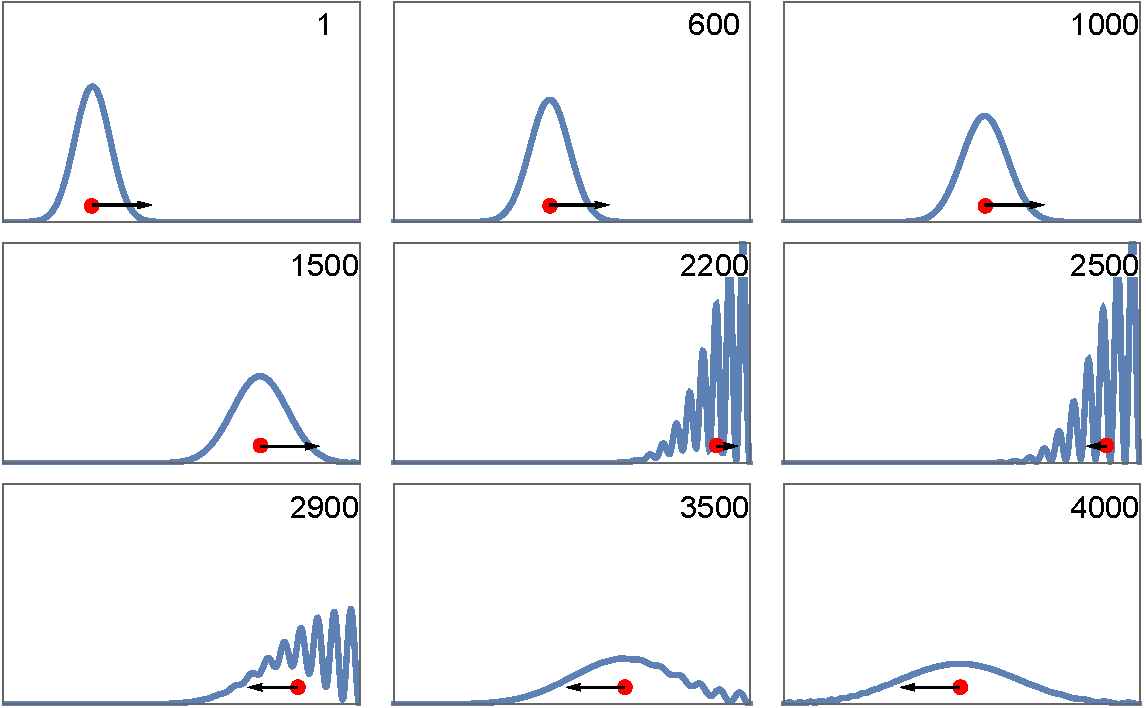
\includegraphics[width=\textwidth]{evolution_1.pdf}
         \caption{\label{fig:evolution_1}}
     \end{subfigure}
     \hfill
     \begin{subfigure}[b]{0.45\textwidth}
         \centering
         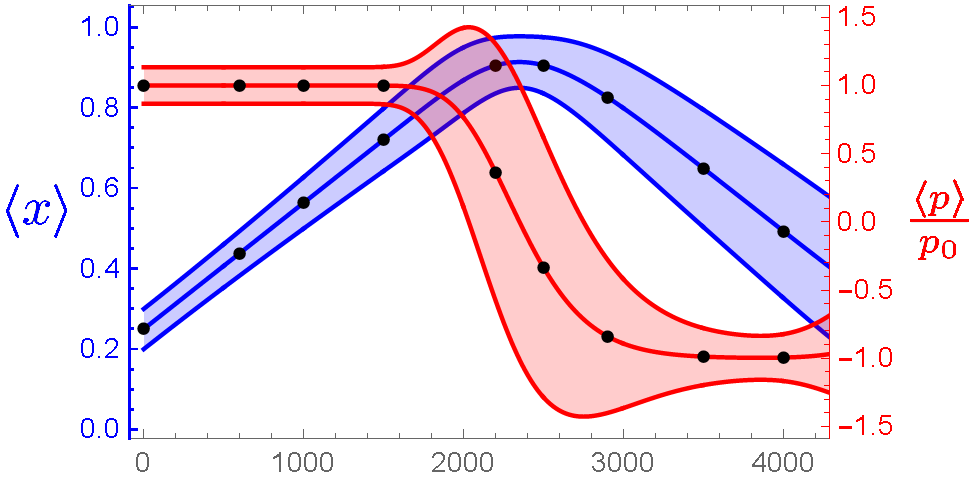
\includegraphics[width=\textwidth]{valores_medios_1.png}
         \caption{\label{fig:valores_medios_1}}
     \end{subfigure}
    \caption{\ref{fig:evolution_1}: evolución temporal de un paquete de ondas gaussiano dentro de una caja de potencial de barreras infinitas. En la sección superior derecha de cada imagen se representa el instante de tiempo correspondiente en unidades de $\delta$. \ref{fig:valores_medios_1}: evolución temporal de la posición media $\langle x \rangle$, el momento medio $\langle p \rangle$ normalizado a tiempo inicial $p_0$ y sus indeterminaciones $\sigma_x$ y $\sigma_p$, respectivamente. Estas últimas se representan como barras de error sombreadas alrededor del valor medio. Los puntos graficados sobre las curvas de $\langle x \rangle$ y $\langle p \rangle$ hacen referencia a los instantes de tiempo graficados en \ref{fig:evolution_1}.}
\end{figure}

También se analizó la evolución temporal de $|\Psi(x,t)|^2$, de los valores medios $\langle x \rangle$ y $\langle p \rangle$ y sus indeterminaciones para cuatro situaciones distintas. En primer lugar, se analizó una partícula en ausencia de barrera ($U_0 = 0$). En la figura \ref{fig:evolution_1} se muestra la evolución temporal de $\mid \Psi \mid^2$ a distintos instantes de tiempo. Además, en la figura \ref{fig:valores_medios_1} se observa la evolución de $\langle x \rangle$, $\langle p \rangle$ y sus indeterminaciones respectivas. Inicialmente el paquete de ondas se desplaza en la dirección de $x$ positivos con incertidumbre $\sigma_x$ creciente. Esto se puede observar en la evolución de $\mid \Psi \mid^2$ como el aumento del ancho del paquete y en la evolución de $\langle x \rangle$ como el aumento de las barras de error. Su crecimiento se puede explicar a partir de la descomposición de la función de onda en ondas planas con distinta velocidad a partir (desarrollo de Fourier). Como existen algunas ondas con mayor velocidad que otras, en la suma total se genera un ensanchamiento del paquete. Sin embargo, la velocidad del grupo es constante y, por lo tanto, $\langle p \rangle$ también lo es. Además, como la energía es constante en el tiempo (figura \ref{fig:energia}) y $\langle V \rangle = 0$, se tiene que $\langle p^2 \rangle = 2 m \langle K \rangle = \langle H \rangle$ es constante. De este modo, a partir de la relación \ref{eq:dispersion}, $\sigma_p$ no cambia durante la propagación inicial del paquete. A partir de $t = 1500$ el paquete comienza a interactuar con la barrera de potencial infinita, reflejándose. La sección incidente de $\Psi(x,t)$ interfiere con la sección reflejada de la misma, produciendo como consecuencia grandes oscilaciones cerca de la pered. En este proceso la indeterminación $\sigma_x$ disminuye debido a que el ancho del paquete disminuye. Físicamente se puede afirmar con mayor certeza dónde está la partícula. Por otro lado, la incerteza $\sigma_p$ aumenta dado que si bien $\langle p^2 \rangle$ es constante, $\langle p \rangle$ disminuye. Otra manera de explicar este comportamiento es a partir de la descomposición en ondas planas discutida anteriormente. Parte de ellas tienen momento lineal en la dirección de $x$ positivos y parte de ellas en la dirección opuesta. Esta gran dispersión en el momento lineal se ve reflejada en un aumento significativo de $\sigma_p$. Por último, a partir de $t = 2900$ se observa que el paquete se desplaza en la dirección de $x$ negativos, ensanchándose progresivamente por el mismo justificativo empleado al inicio de la evolución.

\begin{figure}
     \centering
     \begin{subfigure}[b]{0.45\textwidth}
         \centering
         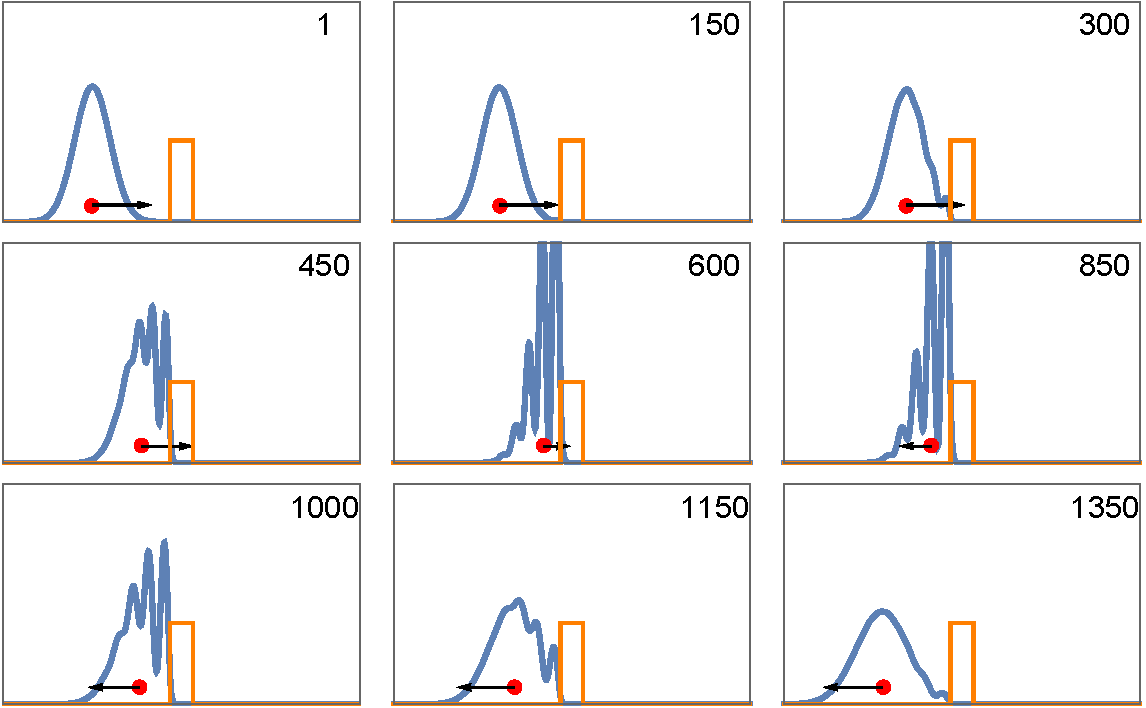
\includegraphics[width=\textwidth]{evolution_2i.pdf}
         \caption{\label{fig:evolution_2i}}
     \end{subfigure}
     \hfill
     \begin{subfigure}[b]{0.45\textwidth}
         \centering
         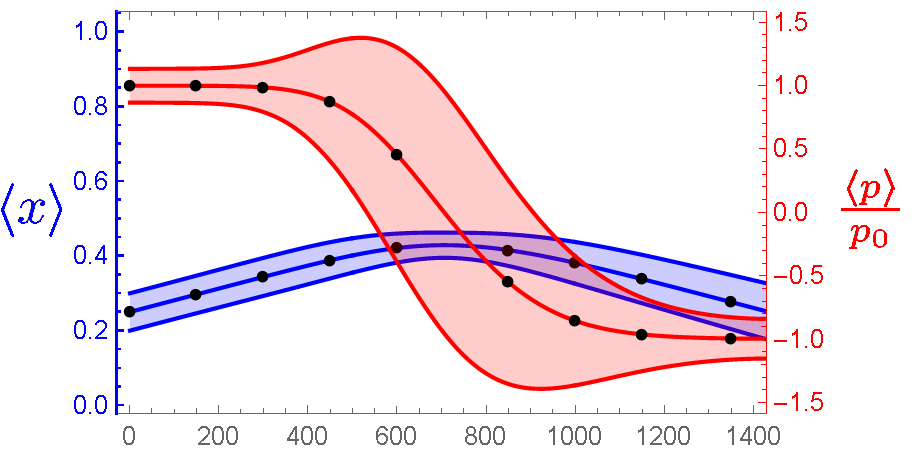
\includegraphics[width=\textwidth]{valores_medios_2i.png}
         \caption{\label{fig:valores_medios_2i}}
     \end{subfigure}
     \caption{\ref{fig:evolution_2i}: evolución temporal de un paquete de ondas gaussiano con momento $k_0^1 = 25 \pi$ en presencia de una barrera de potencial cuadrada. El valor medio de la energía $E_1$ es menor que la altura del potencial $U_0$. En la sección superior derecha de cada imagen se representa el instante de tiempo correspondiente en unidades de $\delta$. \ref{fig:valores_medios_2i}: evolución temporal de la posición media $\langle x \rangle$, el momento medio $\langle p \rangle$ normalizado a tiempo inicial $p_0$ y sus indeterminaciones $\sigma_x$ y $\sigma_p$, respectivamente. Estas últimas se representan como barras de error sombreadas alrededor del valor medio. Los puntos graficados sobre las curvas de $\langle x \rangle$ y $\langle p \rangle$ hacen referencia a los instantes de tiempo graficados en \ref{fig:evolution_2i}.}
\end{figure}

En segundo lugar, se analizó la evolución temporal de una partícula con $k_0^1 = 25 \pi$ y energía $E_1<U_0$. Sólo es de interés la interacción con el potencial $V(x)$ en el interior de la caja, por lo que se discutirá la evolución durante un tiempo menor que en la situación anterior, asegurando que el paquete de ondas no interactúe apreciablemente con las paredes infinitas. Se observa la evolución de $\mid \Psi \mid^2$ en la figura \ref{fig:evolution_2i} y de las cantidades medias y sus indeterminaciones en la figura \ref{fig:valores_medios_2i}. El paquete de ondas se desplaza inicialmente hacia valores positivos de $x$. Al encontrarse con la barrera, interactúa con ella reflejándose y produciendo oscilaciones del mismo modo que en la figura \ref{fig:evolution_1}. Al igual que en la situación anterior, durante este proceso $\sigma_x$ disminuye y $\sigma_p$ aumenta. Esto último se justifica a través del mismo razonamiento expuesto anteriormente considerando que $\langle V \rangle \approx 0$, dado que la función de onda es aproximadamente nula en el interior de la barrera. Luego de este proceso, $\langle p \rangle$ se invierte y el paquete se refleja. Es importante aclarar que realmente existe una pequeña sección de la función de onda que logra atravesar la barrera, pero es tan pequeña que no es observable en la figura \ref{fig:evolution_2i}. Esto implica que existe una probabilidad distinta de cero de encontrar a la partícula a la derecha de la barrera. De este modo se viola el comporamiento clásico en el que una partícula con energía cinética menor al potencial de la barrera no es capaz de atravesarla.

\begin{figure}
     \centering
     \begin{subfigure}[b]{0.45\textwidth}
         \centering
         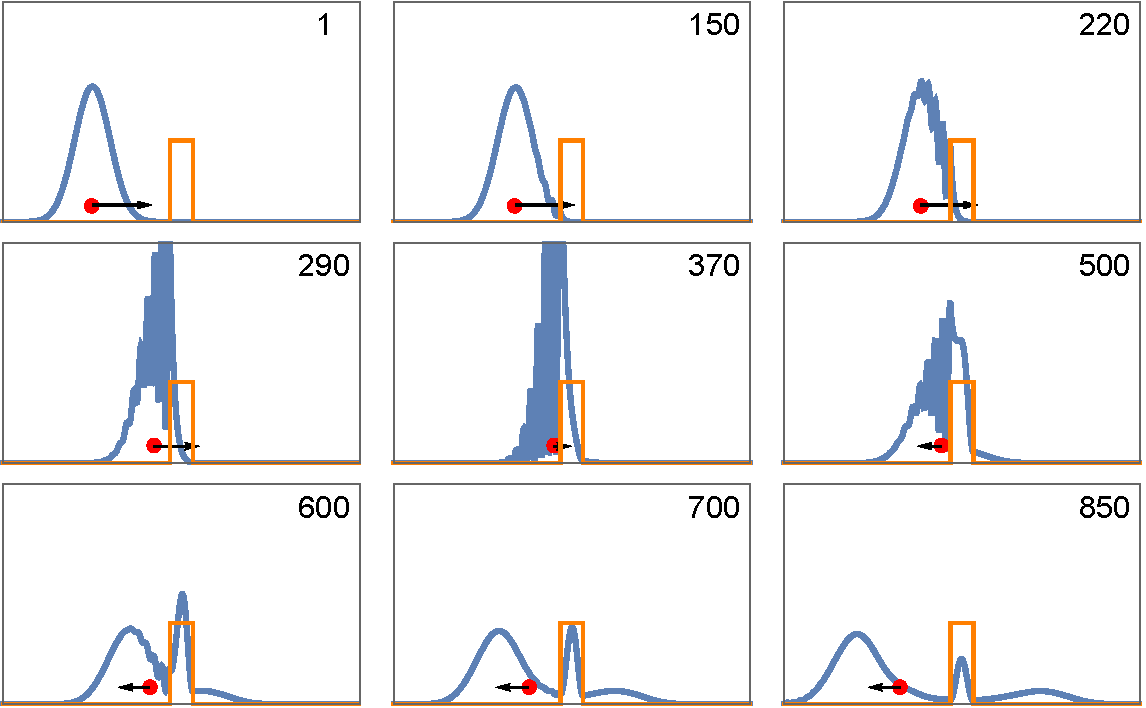
\includegraphics[width=\textwidth]{evolution_2ii.pdf}
         \caption{\label{fig:evolution_2ii}}
     \end{subfigure}
     \hfill
     \begin{subfigure}[b]{0.45\textwidth}
         \centering
         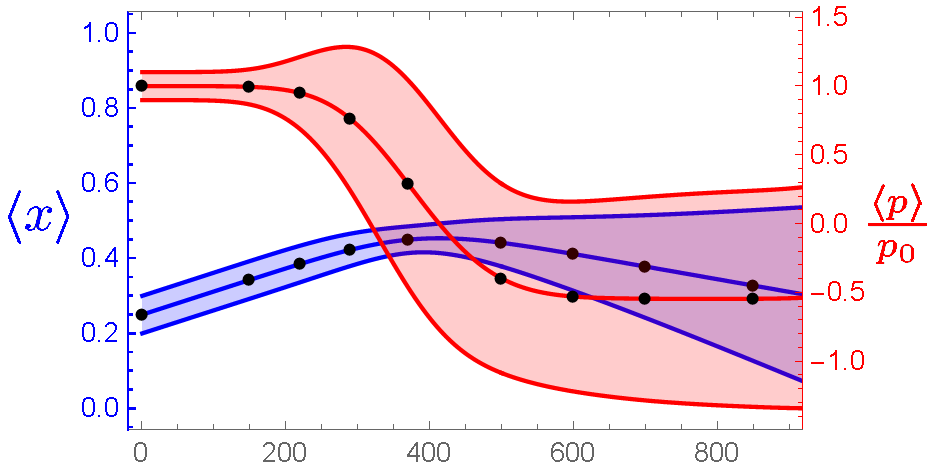
\includegraphics[width=\textwidth]{valores_medios_2ii.png}
         \caption{\label{fig:valores_medios_2ii}}
     \end{subfigure}
     \caption{\ref{fig:evolution_2ii}: evolución temporal de un paquete de ondas gaussiano con momento $k_0^2 = 35 \sqrt{2} \pi$  en presencia de una barrera de potencial cuadrada. El valor medio de la energía $E_2$ es menor pero del mismo orden de magnitud que la altura del potencial $U_0$. En la sección superior derecha de cada imagen se representa el instante de tiempo correspondiente en unidades de $\delta$. \ref{fig:valores_medios_2ii}: evolución temporal de la posición media $\langle x \rangle$, el momento medio $\langle p \rangle$ normalizado a tiempo inicial $p_0$ y sus indeterminaciones $\sigma_x$ y $\sigma_p$, respectivamente. Estas últimas se representan como barras de error sombreadas alrededor del valor medio. Los puntos graficados sobre las curvas de $\langle x \rangle$ y $\langle p \rangle$ hacen referencia a los instantes de tiempo graficados en \ref{fig:evolution_2ii}.}
\end{figure}



En tercer lugar, se estudió la evolución de una partícula con $k_0^2 = 35 \sqrt{2} \pi$ y $E_2 \lesssim U_0$. Se resume gráficamente en las figuras \ref{fig:evolution_2ii} y \ref{fig:valores_medios_2ii}. La diferencia con la situación anterior radica en la interacción con la barrera a partir de $t = 220$. Como antes, una sección de la función de onda se refleja interfiriendo consigo misma y produciendo consecuentemente grandes oscilaciones. Pero además ocurren tres fenómenos nuevos. El primero de ellos es que parte de la onda logra ingresar en la barrera de potencial, como claramente se observa en $t = 290$. El segundo de ellos es que parte de la onda se logra transmitir a pesar de que la partícula posea menor energía que la barrera, como se muestra a partir de $t = 500$. Este fenómeno se denomina tunelamiento cuántico y, como semencionó anteriormente, escapa de la descripción clásica de las partículas. El tercer aspecto de interés es que se logra capturar parte de la función de onda dentro de la barrera. Esto se debe a que la sección de onda que ingresó dentro la misma se refleja constantemente con las paredes con una probabilidad pequeña de transmitir desde el interior. De este modo, la onda queda capturada durante un período de tiempo. En cuanto a $\langle x \rangle$ y $\langle p \rangle$, se encuentran determinados por la onda reflejada dado que esta concentra la mayor parte de la densidad de probabilidad. Por otro lado, sus indeterminaciones $\sigma_x$ y $\sigma_p$ crecen continuamente. No es posible afirmar con certeza dónde está la partícula dado que $\Psi(x,t)$ es apreciablemente no nula en gran parte de $x$ y tampoco se puede afirmar el valor del momento lineal de la misma ya que está constituída por ondas que se desplazan en distintas direcciones.

\begin{figure}
     \centering
     \begin{subfigure}[b]{0.45\textwidth}
         \centering
         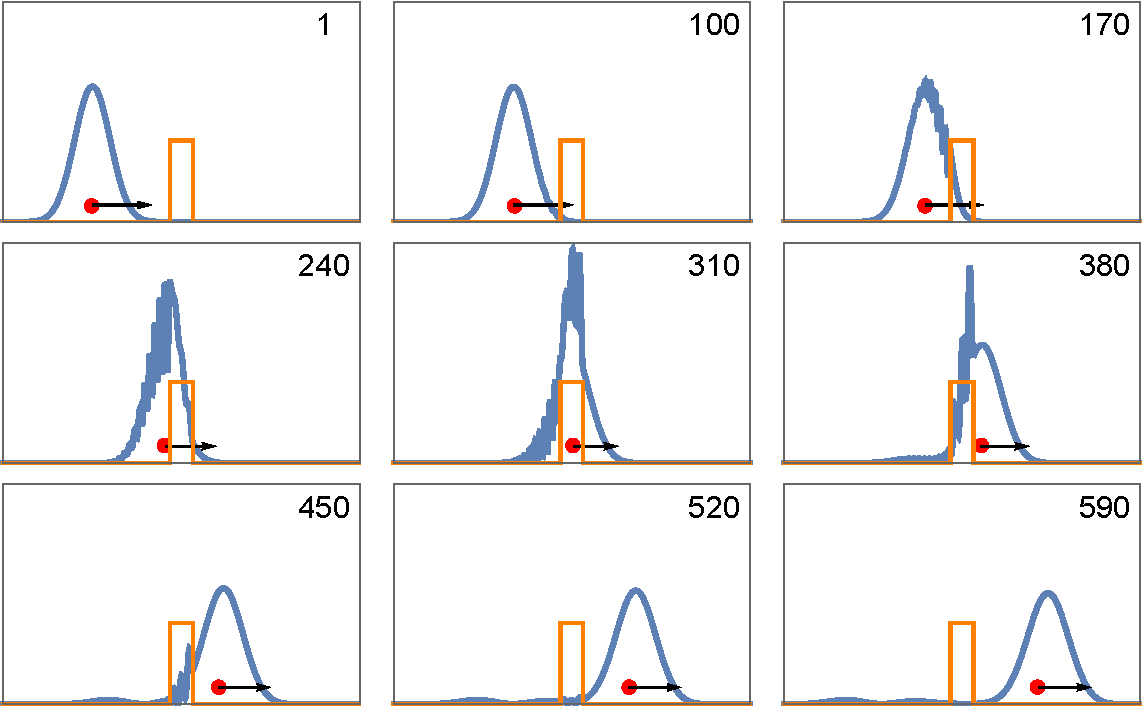
\includegraphics[width=\textwidth]{evolution_2iii.pdf}
         \caption{\label{fig:evolution_2iii}}
     \end{subfigure}
     \hfill
     \begin{subfigure}[b]{0.45\textwidth}
         \centering
         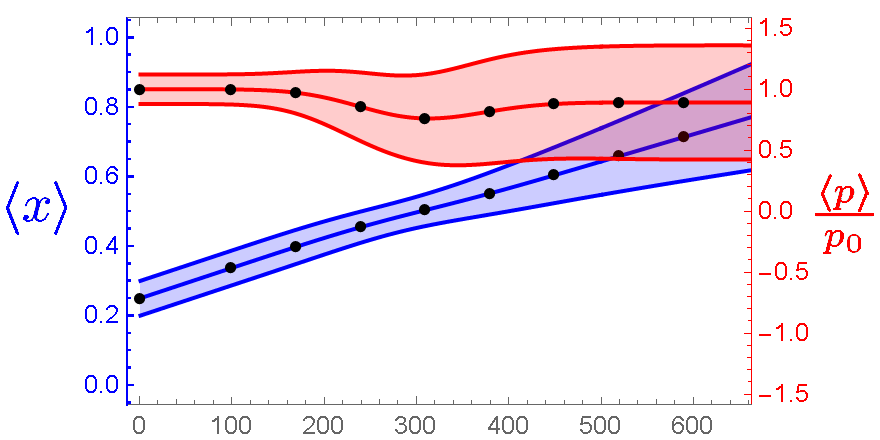
\includegraphics[width=\textwidth]{valores_medios_2iii.png}
         \caption{\label{fig:valores_medios_2iii}}
     \end{subfigure}
     \caption{\ref{fig:evolution_2iii}: evolución temporal de un paquete de ondas gaussiano con momento $k_0^2 = 50 \sqrt{2} \pi$  en presencia de una barrera de potencial cuadrada. El valor medio de la energía $E_3$ es mayor que la altura del potencial $U_0$. En la sección superior derecha de cada imagen se representa el instante de tiempo correspondiente en unidades de $\delta$. \ref{fig:valores_medios_2iii}: evolución temporal de la posición media $\langle x \rangle$, el momento medio $\langle p \rangle$ normalizado a tiempo inicial $p_0$ y sus indeterminaciones $\sigma_x$ y $\sigma_p$, respectivamente. Estas últimas se representan como barras de error sombreadas alrededor del valor medio. Los puntos graficados sobre las curvas de $\langle x \rangle$ y $\langle p \rangle$ hacen referencia a los instantes de tiempo graficados en \ref{fig:evolution_2iii}.}
\end{figure}

En cuarto lugar, se analizó la evolución de una partícula con $k_0^3 = 50 \sqrt{2} \pi$ y $E_3 > U_0$. Se resume gráficamente en las figuras \ref{fig:evolution_2iii} y \ref{fig:valores_medios_2iii}. Al igual que antes, una sección de la onda se captura en el interior de la barrera, otra se transmite y otra se refleja, produciendo indeterminaciones $\sigma_x$ y $\sigma_p$ crecientes con las mismas justificaciones que en el caso anterior. Sin embargo, a diferencia de este último, la sección transmitida es mucho mayor que la reflejada y la capturada y, consecuentemente, $\langle p \rangle$ se mantiene positivo y $\langle x \rangle$ crece continuamente. Esta situación es similar al comportamiento clásico en el que una partícula atraviesa una barrera si posee mayor energía que la misma. De este modo, se esperaría recuperar el resultado clásico a energías $E$ mucho mayores que $U_0$.


\section{Conclusión}

Se resolvió numéricamente la ecuación de Schrödinger unidimensional empleando el método de Crank-Nicholson sobre una grilla discreta de tamaño $T \times L$ con $L = 1$ y $T \lesssim L/(2 \hbar k_0)$ con discretización temporal $\delta = 2 \epsilon^2 / \hbar = 2*10^{-6}$ y discretización espacial $\epsilon = 0.001 \hbar = 0.001$. Se empleó como condición inicial un paquete gaussiano con $x_0 = 0.25$, $\sigma_0 = 0.05$ y distintos momentos $k_0$ que determinan la energía inicial de la partícula. Se emplearon condiciones de borde nulas correspondientes a una caja con barreras de potencial infinito. En cuanto al potencial en la zona interior se consideró una barrera de potencial de ancho $2 a = 0.064$ y distintas alturas $U_0$. Se analizaron cuatro situaciones: una partícula en ausencia de barrera ($U_0 = 0$) con momento $k_0^0 = 25 \pi$ y una partícula en presencia de barrera ($U_0 = (50 \pi)^2$) con tres valores distintos de momento $k_0^1 = 25 \pi$, $k_0^2 = 35 \sqrt{2} \pi$ y $k_0^3 = 50 \sqrt{2} \pi$ correspondientes a energías $E_1 = (25.2 \pi)^2 < U_0$, $E_2 = (49.6 \pi)^2 \lesssim U_0$ y $E_3 = (70.6 \pi)^2  > U_0$, respectivamente. Se corroboró en todos los casos la conservación de la norma, consecuencia directa del uso de la representación de Cayley para el operador de evolución temporal, y de la energía. En cuanto a esta última, se obtuvieron valores de energía distintos a los valores teóricos predichos por la expresión $E = (\hbar k_0)^2$, diferencia que se podría atribuir a la discretización realizada. También se analizó la evolución temporal de la función de onda, de la posición y momento lineal medios y sus indeterminaciones, caracterizando cualitativamente su comportamiento en distintos instantes de tiempo. Para la partícula en ausencia de barrera de potencial se observó la reflexión de la partícula con las paredes de potencial infinito. Para la partícula en presencia de barrera de potencial se obtuvo para $E_1 < U_0$ una reflexión casi completa representando fenomenológicamente el comporamiento clásico esperado. En cambio, para $E \lesssim U_0$  se obtuvo reflexión y transmisión de la onda representando el fenómeno de tunelamiento cuántico. Por último, para $E > U_0$ se recupera el comporamiento clásico con una transmisión casi completa de la función de onda.

\bibliography{Chehade__Schrodinger_tpfinal}



\end{document}

